\chapter{Generieren der Erkennungsregeln}
\label{generierung}

Ziel des Semantic-Liftings ist es, die low-level Änderungen der technischen Differenz wieder einer
bestimmten Editieroperation zuzuordnen. Die Änderungen einer Editieroperation werden durch die
Editierregeln vorgegeben. Das Auslesen der Editieroperation aus der Differenz wird durch die s.g.
Erkennungsregeln erledigt. Eine Erkennungsregel ordnet den low-level Änderungen wieder eine
Editieroperation zu und gruppieren diese in s.g. Semantic-Change-Sets. Die Erkennungsregeln sind,
genau so wie die Editierregel, Henshin Transformationssysteme. Alle Informationen, die für die
Erkennung der Editieroperation benötigt werden, sind in der Editierregel vorhanden und deren
Semantik ist wohldefiniert. Für jeden Teil einer Editierregel lässt sich eindeutig nachvollziehen,
welche Änderungen dadurch in der Differenz auftreten werden. Daher können die Erkennungsregeln
vollständig automatisch aus den Editierregeln generiert werden. Diese Aufgabe übernimmt der
\textbf{Erkennungsregel Generator}.
\begin{quote}
"`Change set recognition rules are getting complex very quickly. However, they are very schematic
and can be automatically generated from their corresponding edit rule."' \cite{KeKT2011ASE} (S.6)
\end{quote}

\section{Implizite Kanten}
\label{implicit_edge}

Bevor die eigentliche Generierung der Erkennungsregel beginnen kann, muss die Editierregel ggf. noch
um bestimmte Kanten erweitert werden. In Ecore kann einer Referenz eine entgegen gerichtete Referenz
(\texttt{eOpposite}) zugeordnet werden. In den meisten Fällen reicht es in Henshin aus, wenn eine
Referenz nur in eine Richtung angegeben wird. Die entgegen gerichtete Referenz wird dann, z.B. beim
erzeugen einer Referenz, automatisch mit eingefügt.

\begin{figure}[htbp]
  \centering
  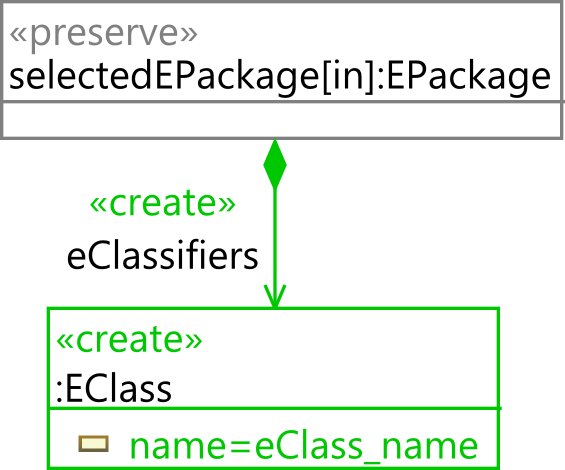
\includegraphics[scale=0.8]{images/add_eclass.png}
  \caption{Ecore Klasse einfügen}
  \label{fig:add_eclass}
\end{figure}

Im Beispiel in Abbildung \ref{fig:add_eclass} wird eine neue Klasse in ein Paket eingefügt. Beim
einfügen neuer Objekte in ein Ecore Modell wird typischerweise eine Referenz sowohl zwischen
Container und Objekt als auch zwischen Objekt und Container erzeugt. Angegeben wurde in diesem Fall
aber nur die Referenz \texttt{eClassifiers} vom Container zum Objekt. Diese Referenz besitzt aber
eine entgegen gerichtete Referenz \texttt{ePackage} vom Objekt zum Container. Eben genau diese
low-level Änderungen werden nach Anwendung dieser Regel in der technischen Differenz auftreten: 2
$\times$ Add-References und 1 $\times$ Add-Object.

Das Problem solcher \textbf{impliziten Kanten} kann wie schon angedeutet in Ecore häufiger
auftreten. Damit alle Änderungen durch die Erkennungsregel wieder vollständig zugeordnet werden
können, müssen zunächst alle impliziten Kanten in den Transformationsgraphen eingefügt werden. Dazu
werden folgende Schritte für alle Kanten im Graphen ausgeführt:

\begin{enumerate}
  \item Besitzt der Typ (\texttt{EReference}) der aktuellen Kante $X$ eine entgegen gerichtete
  Referenz (\texttt{eOpposite})?
  \item Ist dies der Fall, dann überprüfe, ob eine Kante $Y$ existiert, die in entgegengesetzter
  Richtung zur Kante $X$ verläuft und vom entsprechenden \texttt{eOpposite} Typ ist.
   \item Wurde Kante $Y$ nicht gefunden, dann füge sie dem Graphen hinzu.
\end{enumerate}
Nachdem alle impliziten Kanten eingefügt wurden, kann mit der eigentlichen Erkennungsregel
Generierung begonnen werden.

\section{Parameter}
\label{parameter}

Die Parameter der Editierregel werden zu Beginn vollständig in die Erkennungsregel übernommen. Sie
lassen sich dabei in zwei Kategorien einteilen:

\begin{itemize}
  \item \textbf{Regel-Parameter:} Parameter wird innerhalb der Regel durch ein Attribut eines Knoten
  initialisiert.
  \item \textbf{Unit-Parameter:} Parameter wird von außen an die Regel übergeben. D.h es wird ein
  benutzerdefinierter Wert vor Aufruf der Regel gesetzt. Dies ist im Fall einer EMF-Refactor
  Regel immer ein Parameter, der auf einen Parameter der  \textit{mainUnit} gemappt wurde.
\end{itemize}
Diese Unterscheidung spielt innerhalb der Erkennungsregel beim vergleichen der Attributwerte eine
Rolle. Der ursprüngliche Wert eines Unit-Parameters, der der Editierregel übergeben wurde, ist in
der Erkennungsregel nicht mehr bekannt. Problematisch wird dies dann, wenn der Wert des Unit-Parameters
durch einen bestimmten Ausdruck mit anderen Parametern oder Werten verrechnet wurde (z.B.
\texttt{+,-,*,/}). Um den Wert des Unit-Parameter wieder zu extrahieren, würde man die entsprechende
Umkehrfunktion zu diesem Ausdruck benötigen, bzw. man müsste diesen automatisch berechnen. In
Henshin ist es allerdings nur möglich, Attributwerte auf einfache Gleichheit zu überprüfen. Reguläre
Ausdrücke oder ähnliches, um z.B. eine String Konkatenation zu überprüfen, sind nicht möglich.
Ausdrücke in denen Unit-Parameter verrechnet werden, werden daher bei der Generierung bisher
übergangen.

\section{Generierungsmuster}
\label{patterns}

Um aus einer Editierregel eine Erkennungsregel zu generieren, werden jeweils die einzelnen Elemente
eines Henshin Transformationssystems betrachtet. Ein Transformationssystem besteht aus einem linken
(\textit{Left-Hand Site} (LHS)) und einem rechten Graph (\textit{Right-Hand Site} (RHS)). Dieser
besitzt wiederum: Knoten (\textit{engl. Node}), Kanten (\textit{engl. Edge}) und Attribute
(\textit{engl. Attribute}). Alle diese Elemente können sowohl nur auf der linken
(\texttt{<<delete>>}) als auch nur auf der rechten Seite (\texttt{<<create>>}) oder auch auf beiden
Seiten (\texttt{<<preserve>>})  der Regel vorkommen. Diese Stereotype werden im Folgenden verwendet,
um die Zuordnung eines Henshin Elements zu einer bestimmten Seite der Regel auszudrücken. In der
grafischen Henshin Notation dargestellt ergeben sich damit die folgenden Muster, um Elemente einer
Editierregel in eine Erkennungsregel zu transformieren. Die Editierregel Muster sind jeweils links
und die Erkennungsregel-Muster jeweils rechts dargestellt. Das fiktive Metamodell in Abbildung
\ref{fiktiv_metamodel} dient als Beispiel für die abgebildeten Muster.

\begin{figure}[htbp]
  \centering
  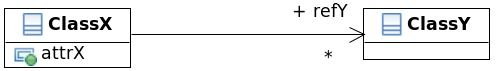
\includegraphics[scale=0.65]{images/fiktiv_metamodel.png}
  \caption{Fiktives Metamodell}
  \label{fiktiv_metamodel}
\end{figure}

\begin{itemize}
  \item \textbf{Remove-Object-Pattern:} Für jeden Knoten, der nur auf der linken Seite der Regel
  vorkommt, wird das Muster in Abbildung \ref{pattern_remove_object} erzeugt. Ein Remove-Object
  zeigt auf ein Objekt aus Modell A vom entsprechenden Typ.
  
  \begin{figure}[htbp]
    \centering
    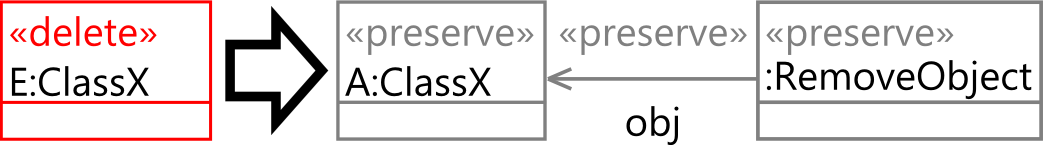
\includegraphics[scale=0.8]{images/pattern_remove_object.png}
    \caption{Remove-Object-Pattern}
    \label{pattern_remove_object}
  \end{figure}
  
  \item  \textbf{Add-Object-Pattern:} Analog zum Remove-Object-Pattern wird das Add-Object-Pattern
  für jeden Knoten angelegt, der nur auf der rechten Seite der Regel vorkommt. Das referenzierte
  Objekt ist in diesem Fall aus Modell B.
  
  \begin{figure}[htbp]
    \centering
    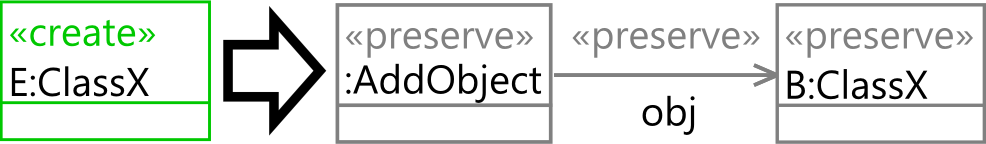
\includegraphics[scale=0.8]{images/pattern_add_object.png}
    \caption{Add-Object-Pattern}
  \end{figure}
  
  \item \textbf{Correspondence-Pattern:} Innerhalb der Differenz werden durch dieses Muster genau
  die Teile ausgewählt, die sich von Modell A zu Modell B nicht verändert haben. Dazu wird durch
  einen \textbf{Correspondence-Knoten} ein Objekt aus Modell A mit dem entsprechenden Objekt aus
  Modell B verbunden. Siehe Abbildung \ref{fig:pattern_correspondence}. Dieses Muster tritt immer
  dann auf,  wenn ein Knoten auf beiden Seiten der Editierregel vorkommt (\texttt{<<preserve>>}).
  Knoten, die Objekte aus Modell A bzw. Modell B repräsentieren, werden im Folgenden als
  \textbf{Modell A Knoten} bzw. \textbf{Modell B Knoten} bezeichnet.
  
  \item \textbf{Preserved-Reference-Pattern:} Genau so wie \texttt{<<preserve>>} Knoten in der
  Editierregel durch \texttt{<<preserve>>} Kanten verbunden werden, werden auch die entsprechend
  Modell A und B Knoten der Correspondence-Patterns verbunden.
  
  \begin{figure}[htbp]
    \centering
    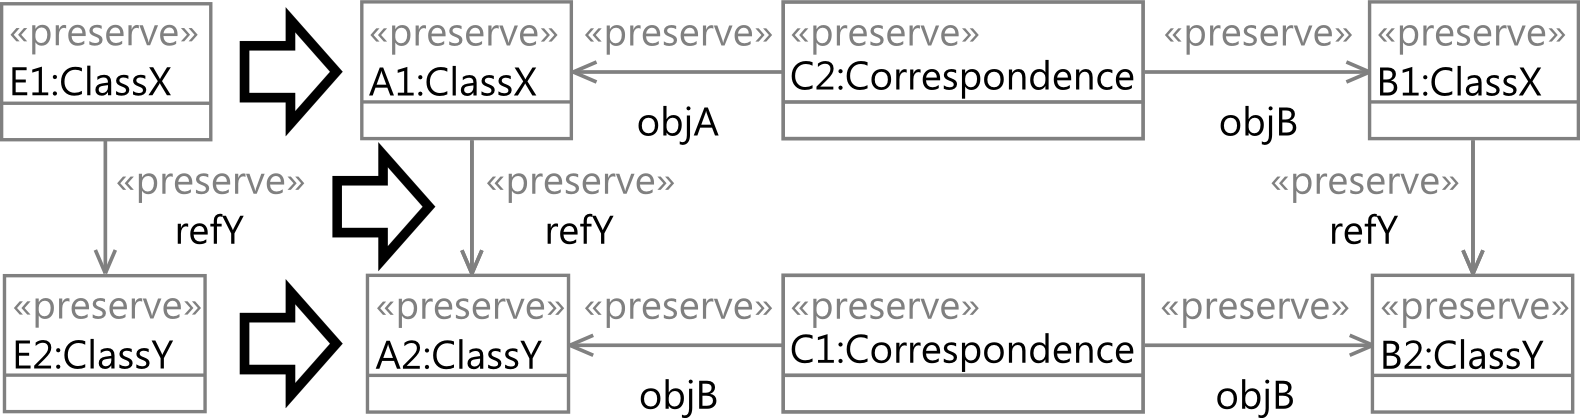
\includegraphics[scale=0.8]{images/pattern_correspondence.png}
    \caption{Correspondence- \& Preserved-Reference-Pattern}
    \label{fig:pattern_correspondence}
  \end{figure}
 
  \item \textbf{Remove-Reference-Pattern:} Als nächstes werden nun die Kanten betrachtet, die nur
  auf der linken Seite (\texttt{<<delete>>}) der Regel  vorkommen. Eine Remove-Reference verbindet durch
  Quelle (\texttt{src}) und Ziel (\texttt{tgt})  immer zwei Modell A Knoten. D.h., werden die Muster
  beim generieren in der hier beschriebenen Reihenfolge abgearbeitet, so wurden die Knoten $A1$ und
  $A2$ bereits durch Correspondence-Patterns oder durch Remove-Object-Patterns erzeugt, da sich die
  Muster an dieser Stelle überschneiden. Welche Muster sich überschneiden, hängt eben davon ab, ob
  die Knoten der Editierregel \texttt{<<preserve>>} oder \texttt{<<delete>>} Knoten sind. Der Fall eines
  \texttt{<<create>>} Knoten in Verbindung mit einer \texttt{<<delete>>} Kante ist nicht möglich und
  muss daher nicht betrachtet werden.
  
  Neben Quelle und Ziel der Editierregel Kante muss in der Erkennungsregel noch der Typ betrachtet
  werden. Dazu wird das Meta-Metamodell, also Ecore, verwendet und der Typ der Remove-Reference auf
  eine \texttt{EReference} mit dem entsprechenden Namen geprüft. Grundsätzlich könnte es vorkommen, dass
  eine Referenz mit dem gleichen Namen im Metamodell mehrfach existiert. Der Kontext für die
  Referenz wird aber eindeutig durch die Quelle (\texttt{src}) der Remove-Reference vorgegeben. Ein
  solcher Knoten zur Überprüfung des Typs wird im Folgenden als \textbf{Typknoten} bezeichnet.
  
  \begin{figure}[htbp]
    \centering
    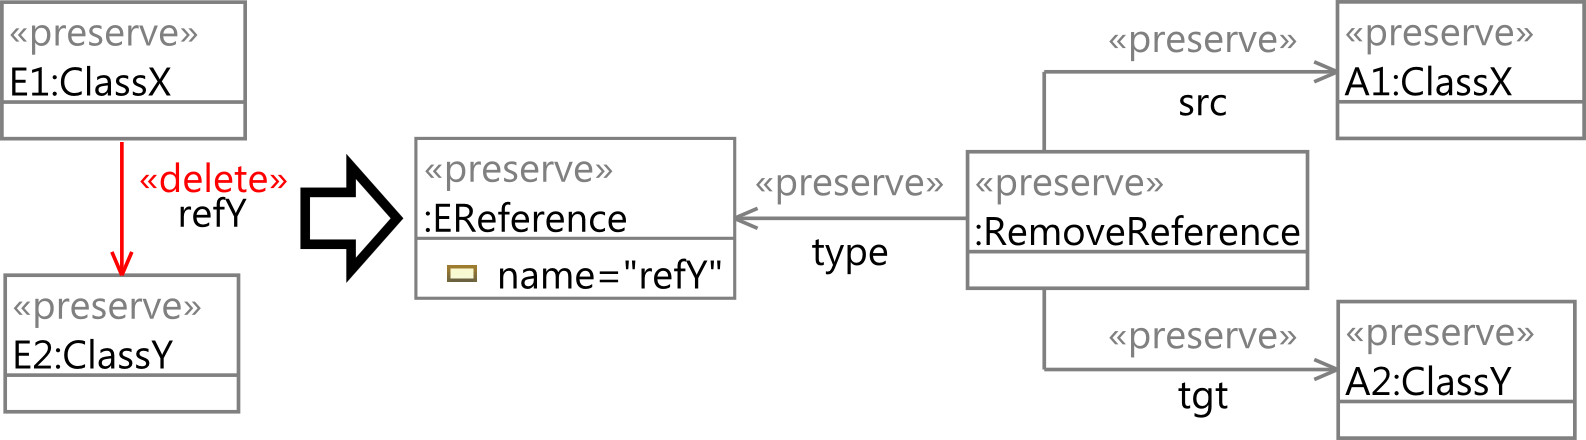
\includegraphics[scale=0.8]{images/pattern_remove_reference.png}
    \caption{Remove-Reference-Pattern}
  \end{figure}
  
  \item \textbf{Add-Reference-Pattern:}  Für das Add-Reference-Pattern werden analog zum
  Remove-Reference-Pattern die Kanten betrachtet, die nur auf der rechten Seite
  (\texttt{<<create>>}) der Editierregel vorkommen.
  
  Innerhalb der Editierregel können \texttt{<<create>>} Kanten nur zwischen \texttt{<<create>>} oder
  \texttt{<<preserve>>} Knoten auftreten.  Damit zeigen die \texttt{src} und \texttt{tgt} Kanten des
  Add-Reference Knoten immer auf Modell B Koten. Entsprechend dem Remove-Reference-Pattern wurden
  die Modell B Knoten $B1$ und $B2$ bereits von Correspondence-Patterns oder von
  Add-Object-Patterns erzeugt.
  
  \begin{figure}[htbp]
    \centering
    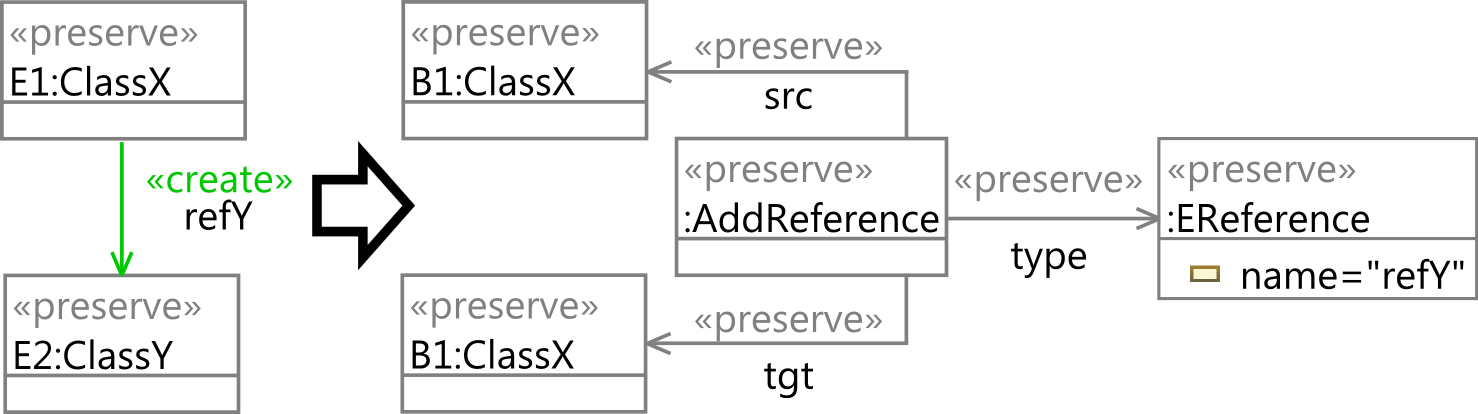
\includegraphics[scale=0.8]{images/pattern_add_reference.png}
    \caption{Add-Reference-Pattern}
  \end{figure}

  \item \textbf{Attribute-Value-Change-Pattern:} Dieses Muster wird nur auf Attribute angewendet,
  die Teil eines \texttt{<<preserve>>} Knoten sind. Für Attribute, die beim neu Anlegen von Objekten
  gesetzt werden, werden bei der Differenz-Ableitung keine Attribute-Value-Changes erzeugt.
  D.h. \texttt{<<create>>} Knoten und deren Attribute müssen nicht beachtet werden.
  
  Daher verbindet das Attribute-Value-Change-Pattern immer ein Objekt aus Modell A mit dem
  entsprechenden Objekt aus Modell B. Das bedeutet für diesen Fall, dass die Knoten $A1$ und $B1$
  bereits durch ein Correspondence-Pattern angelegt wurden. Der Typ des Attributs wird, ähnlich wie
  der Referenztyp beim Remove-Reference-Pattern, durch einen \texttt{EAttribute} Typknoten mit
  Hilfe des Namens überprüft.
  
  \begin{figure}[htbp]
    \centering
    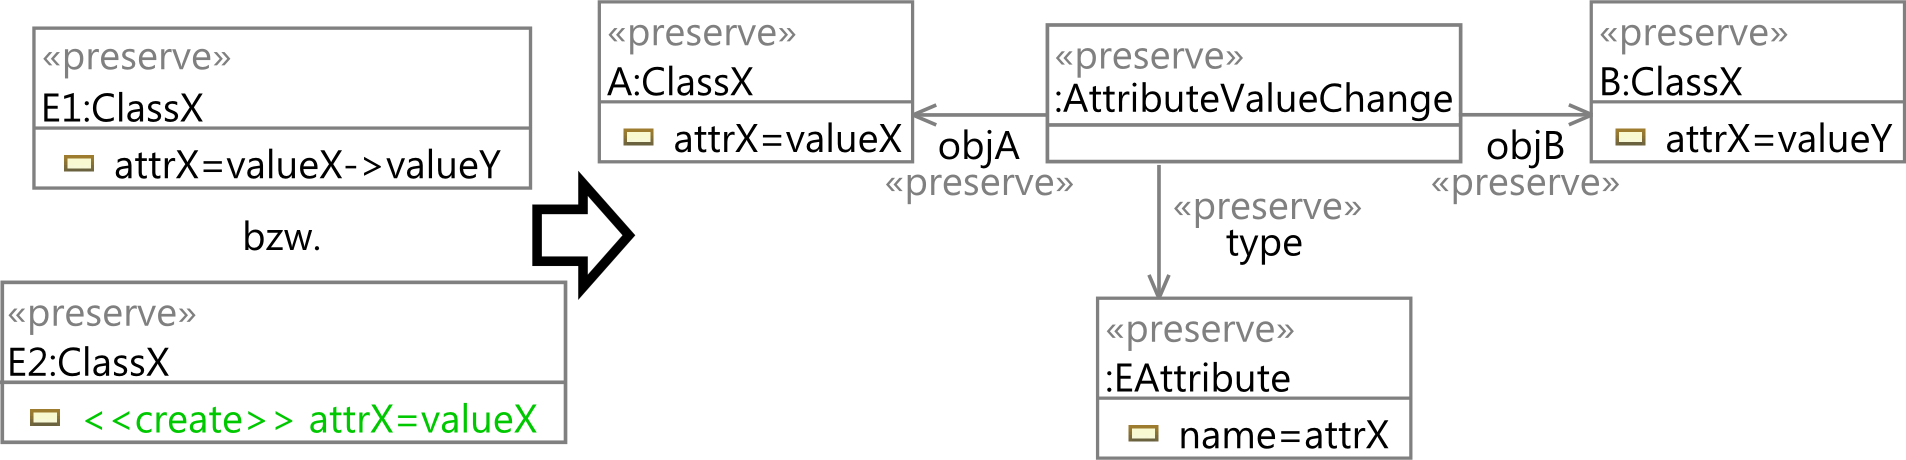
\includegraphics[scale=0.8]{images/pattern_attribute_value_change.png}
    \caption{Attribute-Value-Change-Pattern}
  \end{figure}
  
  Zusätzlich wird in der Erkennungsregel noch der Wert, der in der Editierregel angegebenen
  Attribute überprüft. Handelt es sich um feste primitive Werte, also z.B. Zeichenketten oder
  Zahlen, kann damit im ersten Fall überprüft werden, ob sich der Wert im Modell A Objekt von
  \textit{valueX} zu \textit{valueY} im Modell B Objekt verändert hat. Im zweiten Fall tritt das
  Attribut nur auf der rechten Seite der Regel (\texttt{<<create>>}) auf, hier würde das Attribut
  nur für den Modell A Knoten (Knoten $A1$) angelegt und überprüft.
  
  Handelt es sich hingegen bei den Henshin Attributwerten um Parameter, so würde dadurch bei
  mehrfachem Auftreten eines Parameters in verschiedenen Attributen überprüft, ob die jeweiligen
  Werte gleich sind. Neben einzelnen primitiven Werten und Parametern können für Henshin Attribute
  auch komplexere \textit{JavaScript} Ausdrücke mit Parametern, Werten und Operatoren angelegt
  werden. Für solche Ausdrücke gelten die zuvor im Abschnitt \ref{parameter} beschriebenen
  Einschränkungen für Unit-Parameter. Dies gilt auch für alle folgenden Attribute-Value-Patterns.
  
  \item \textbf{Add-Attribute-Value-Pattern:} Wie bereits erwähnt werden für neu angelegte Objekte
  keine Attribute-Value-Changes berechnet. Das Attribut wird aber wieder für das entsprechende
  Modell B Objekt geprüft.
   
  \begin{figure}[htbp]
    \centering
    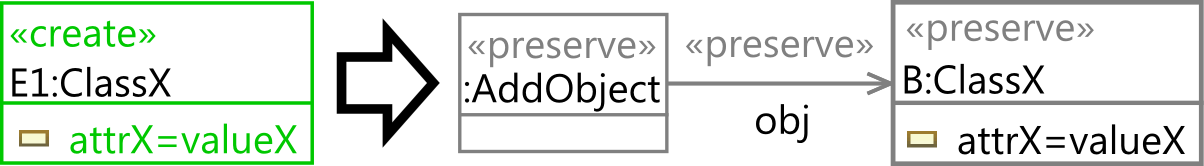
\includegraphics[scale=0.8]{images/pattern_add_attribute_value.png}
    \caption{Add-Attribute-Value-Pattern}
  \end{figure}
   
  \item \textbf{Remove-Attribute-Value-Pattern:} Dieses Muster wird analog zum
  Add-Attri"-bute-Value-Pattern für aus Modell A entfernte Objekte angelegt.
  
  \begin{figure}[htbp]
    \centering
    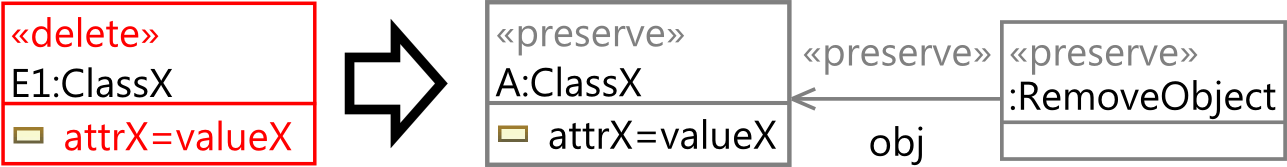
\includegraphics[scale=0.8]{images/pattern_remove_attribute_value.png}
    \caption{Remove-Attribute-Value-Pattern}
  \end{figure}
  
  \item \textbf{Preserved-Attribute-Value-Pattern:} Beim Preserved-Attribute-Value-Pattern wird
  überprüft, dass sich ein Wert von Modell A zu Modell B nicht ändert. Dazu wird das
  gleiche Attribut sowohl für den Modell A  Knoten als auch für Modell B Knoten angelegt. Ein
  \texttt{<<delete>>} Attribut in einem \texttt{<<preserve>>} Knoten verhält sich dabei in Henshin
  ganuso wie ein \texttt{<<preserve>>} Attribut.
  
%   \begin{centering}
%     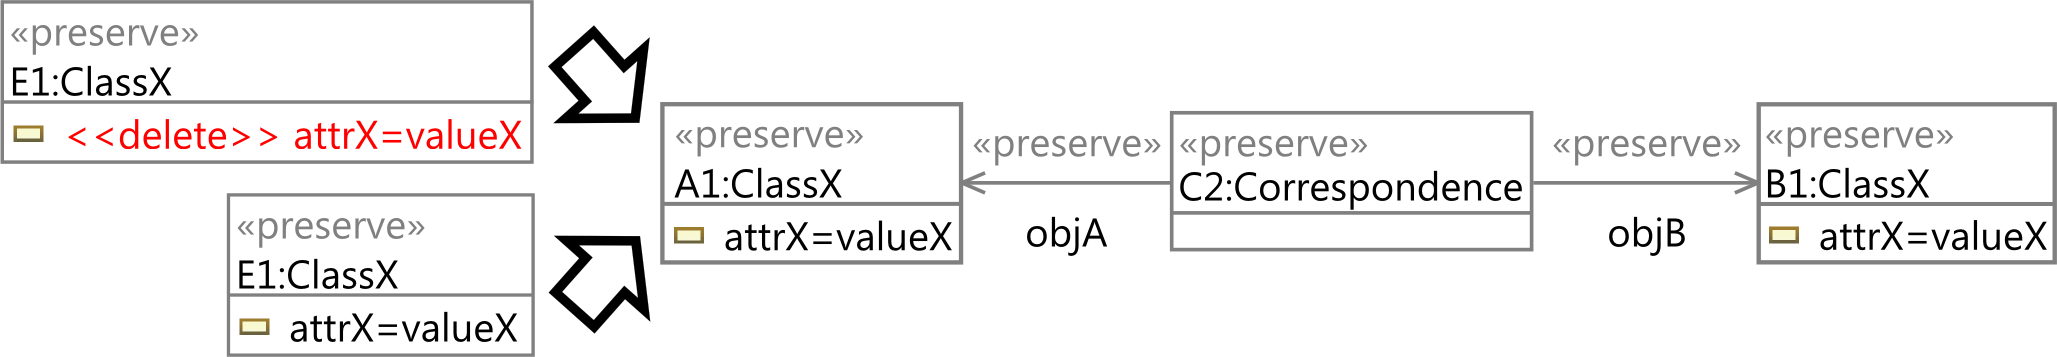
\includegraphics[scale=0.78]{images/pattern_preserve_attribute_value.png}\\
%     \stepcounter{figure}
%     Abbildung \thefigure: Preserved-Attribute-Value-Pattern\\
%   \end{centering}
  
  \begin{figure}[htbp]
    \centering
    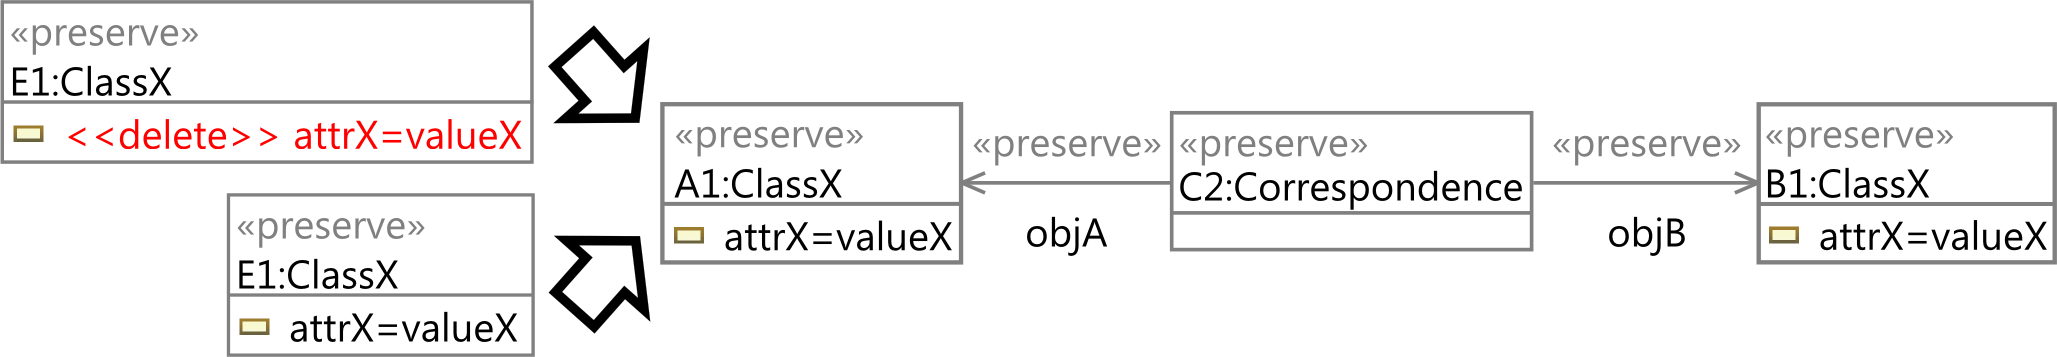
\includegraphics[scale=0.8]{images/pattern_preserve_attribute_value.png}
    \caption{Preserved-Attribute-Value-Pattern}
    \label{avc-preserve}
  \end{figure}
  
  \item \textbf{Semantic-Change-Set-Pattern:} Abschließend muss noch der
  \textbf{Differenz-Kno"-ten} und der \textbf{Semantic-Change-Set-Knoten} angelegt und mit allen \textbf{Änderungsknoten}
  (Add/Remove-Object-Knoten, Add/Remove-Reference-Knoten und Attribute-Value-Change-Knoten)
  verbunden werden. Für das Semantic-Change-Set werden noch die drei folgenden Attribute angelegt und
  initialisiert: \texttt{name}, \texttt{priority} und \texttt{refinementLevel}. Der Name des
  Semantic-Change-Sets entspricht der ursprünglichen Editierregel. Auf die Attribute
  \texttt{priority} und \texttt{refinementLevel} wird später im Rahmen des Abschnitts
  \ref{post_processing} Post-Processing noch genauer eingegangen.

  \begin{figure}[h!]
    \centering
    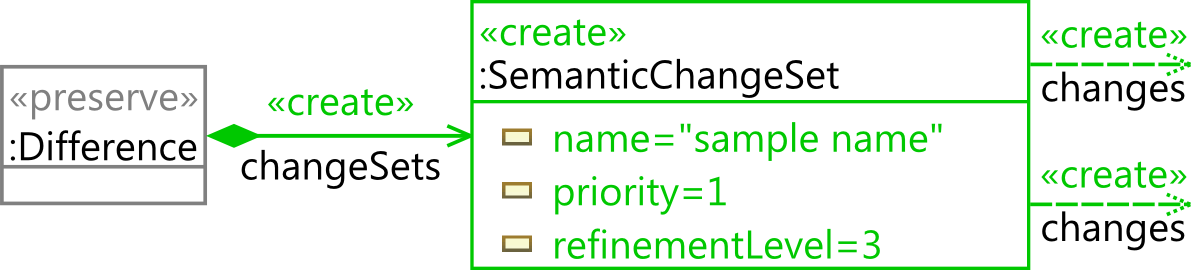
\includegraphics[scale=0.8]{images/pattern_semantic_change_set.png}
    \caption{Semantic-Change-Set-Pattern}
  \end{figure}
  
\end{itemize}

\subsection{Traces}
\label{traces}

Grundsätzlich ist die Reihenfolge, in der die Muster abgearbeitet werden, voneinander unabhängig.
Da die einzelnen Muster aber über die Modell A und B Knoten zusammenhängen, bietet es sich an zunächst
die Remove/Add-Object- und Correspondence-Patterns zu erzeugen. Damit eine korrekte Zuordnung der
sich überschneidenden Knoten zwischen den einzelnen Muster möglich ist, muss abgespeichert werden,
welcher Modell A und B Knoten der Erkennungsregel welchem Knoten der Editierregel entspricht. Diese
Zugehörigkeit von Knoten wird im Folgenden als \textbf{Trace} bezeichnet.

\subsection{Typknoten}
\label{typknoten}

Eine weitere Überschneidung kann bei den Typknoten der Remove-Reference-Patterns und
Add-Reference-Patterns oder beim Attribute-Value-Change-Pattern auftreten. Da der Henshin Graph
injektiv auf den Arbeitsgraphen abgebildet wird, darf auch jeder Typknoten, der ein bestimmtes
Element des Metamodells darstellt, nur einmal erzeugt werden. 

\subsection{Generierungsbeispiel}
\label{gen_example}

Die Muster müssen auf alle Elemente in einer Editierregel angewandt werden, um die zugehörige
Erkennungsregel zu generieren. In Abbildung \ref{fig:add_eclass_recognition} ist die generierte
Erkennungsregel (unten) zu der Editierregel \textit{add empty EClass} (oben) abgebildet. In diesem
Fall lassen sich vier Generierungsmuster identifizieren:

\begin{itemize}
  \item 1 $\times$ Correspondence-Pattern markiert mit (1).
  \item 2 $\times$ Add-Reference-Pattern. Die Referenz \texttt{eClassifiers} wurde mit (2) markiert.
  Die Referenz \texttt{ePackage} ist eine implizite Kante und daher nicht in der Editierregel zu sehen.
  \item 1 $\times$ Add-Object-Pattern markiert mit (3).
\end{itemize}

\begin{figure}[htbp]
  \centering
  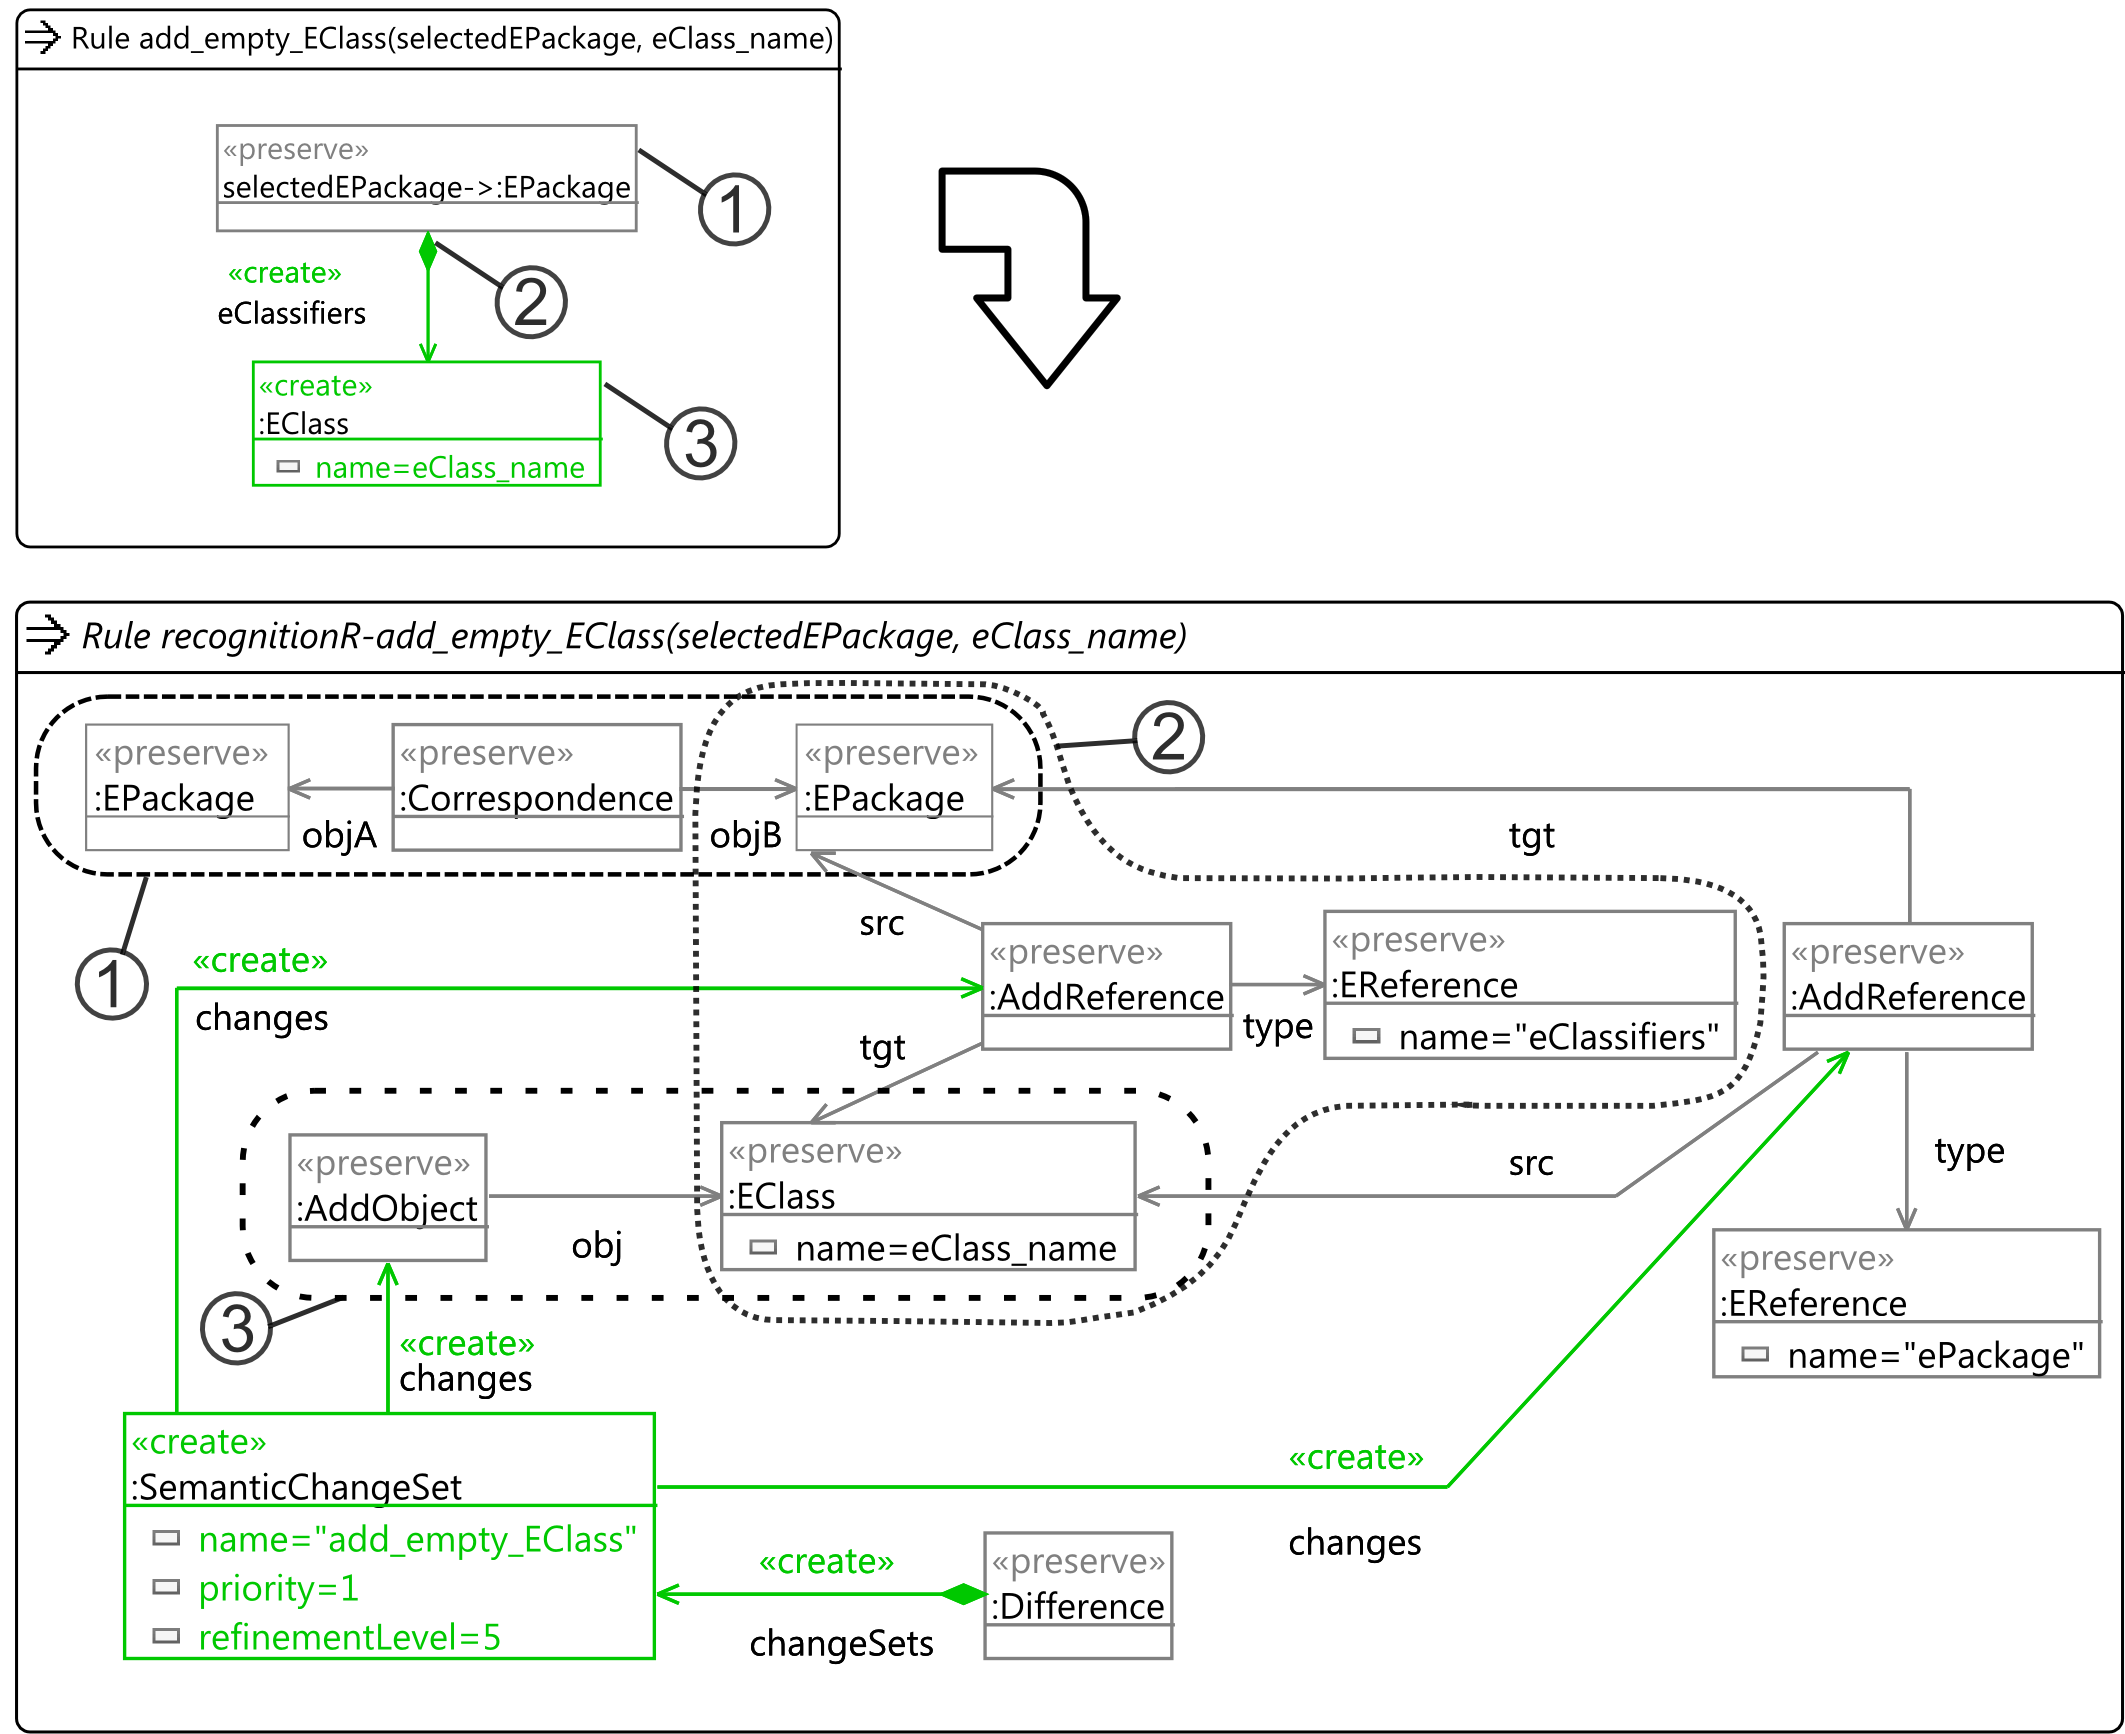
\includegraphics[width=1.0\textwidth]{images/add_eclass_recognition.png}
  \caption{Add \texttt{EClass} Erkennungsregel}
  \label{fig:add_eclass_recognition}
\end{figure}

% Dazu werden bei der Generierung alle bereits erzeugten Typknoten in einer Liste abgespeichert,
% sodass nur bei Bedarf neue Typknoten angelegt werden.

\section{Amalgamation Units}

Eine Amalgamation Unit besteht immer aus genau einer Kernregel und beliebig vielen Multiregeln.
Um eine Amalgamation Unit von einer Editierregel in eine Erkennungsregel zu transformieren, muss
die Kernregel und jede einzelne Multiregel nach dem zuvor beschriebenen Verfahren in eine
Erkennungsregel transformiert werden. \texttt{editR2RecognR()} im Pseudocode in Abbildung
\ref{fig:amalgamtion_code}

\begin{figure}[htbp]
  \centering
  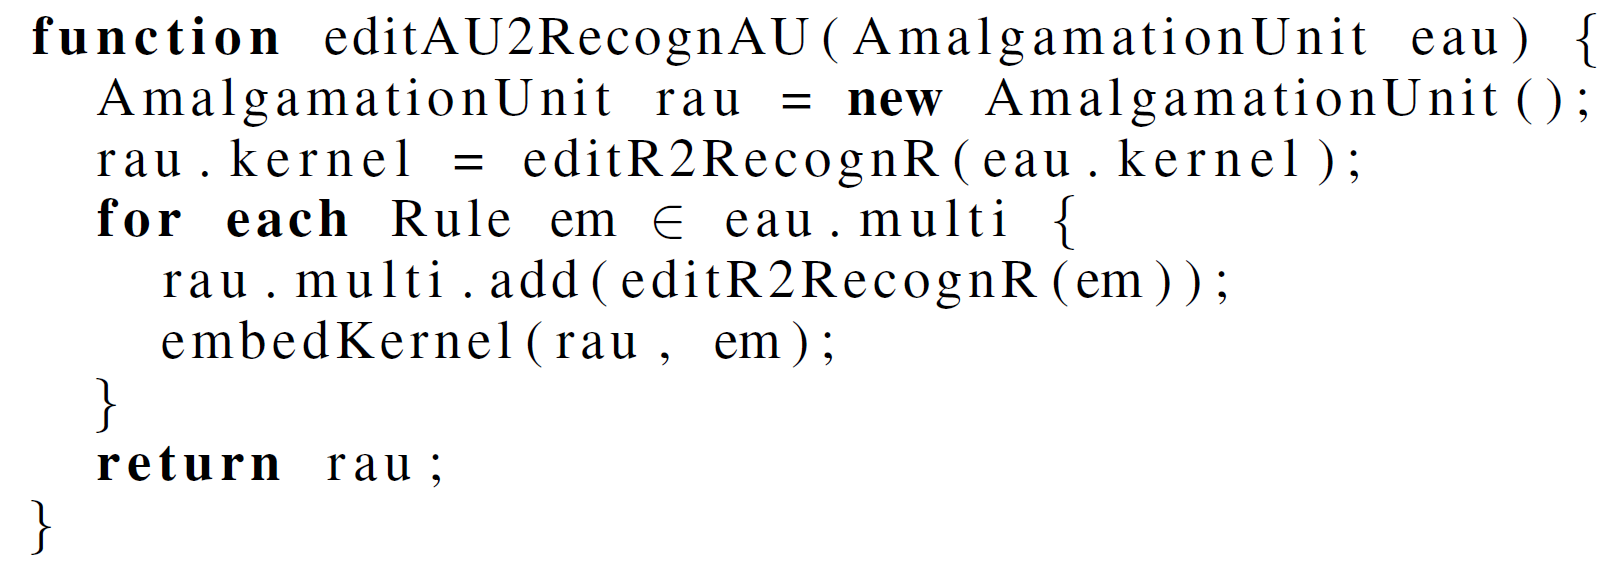
\includegraphics[scale=0.18]{images/amalgamation_code.png}
  \caption{Amalgamation Unit Generierung \cite{KeKT2011ASE} (S.7)}
  \label{fig:amalgamtion_code}
\end{figure}

Der nächste Schritt ist dann das Erzeugen der Mappings zwischen Kernregel und Multiregeln.
\texttt{embedKernel()} im Pseudocode in Abbildung \ref{fig:amalgamtion_code}. D.h.
für jeden Knoten einer Multi-Erkennungsregel wird ein Mapping auf einen Knoten der
Kern-Erkennungsregel angelegt. Das Mapping zwischen einer Multi-Erkennungsregel und einer
Kern-Erken"-nungsregel lässt sich nur dann vollständig angeben, wenn die entsprechende
Multi-Editierregel die Kern-Editierregel als Teilgraph enthält. Dies gilt sowohl für Knoten als
auch für Kanten.

Das Problem beim Anlegen der Mappings besteht darin, dass aus einem Knoten einer Editierregel immer
mehrere Knoten in der Erkennungsregel resultieren. Für alle Kanten besteht das gleiche Problem.
Außerdem existieren für Kanten keine expliziten Mappings. Es wäre also rein technisch nicht
unmöglich in einer Multiregel eine Kante anzulegen, die nicht in der Kernregel vorkommt. Dies würde
aber bei der Generierung zu einigen technischen Problemen führen und ist deshalb zu vermeiden.
Grundsätzlich wird dadurch die Funktionalität der Amalgamation Unit auch nicht eingeschränkt. Dies
lässt sich nachvollziehen, wenn man bedenkt, dass beim Ausführen einer Amalgamation Unit die
Multiregel im Prinzip mit der Kernregel (mehrfach) verschmolzen wird. Es spielt daher keine Rolle,
ob eine Kante der Multiregel zuvor in der Kernregel vorhanden war oder nicht.

\begin{figure}[htbp]
  \centering
  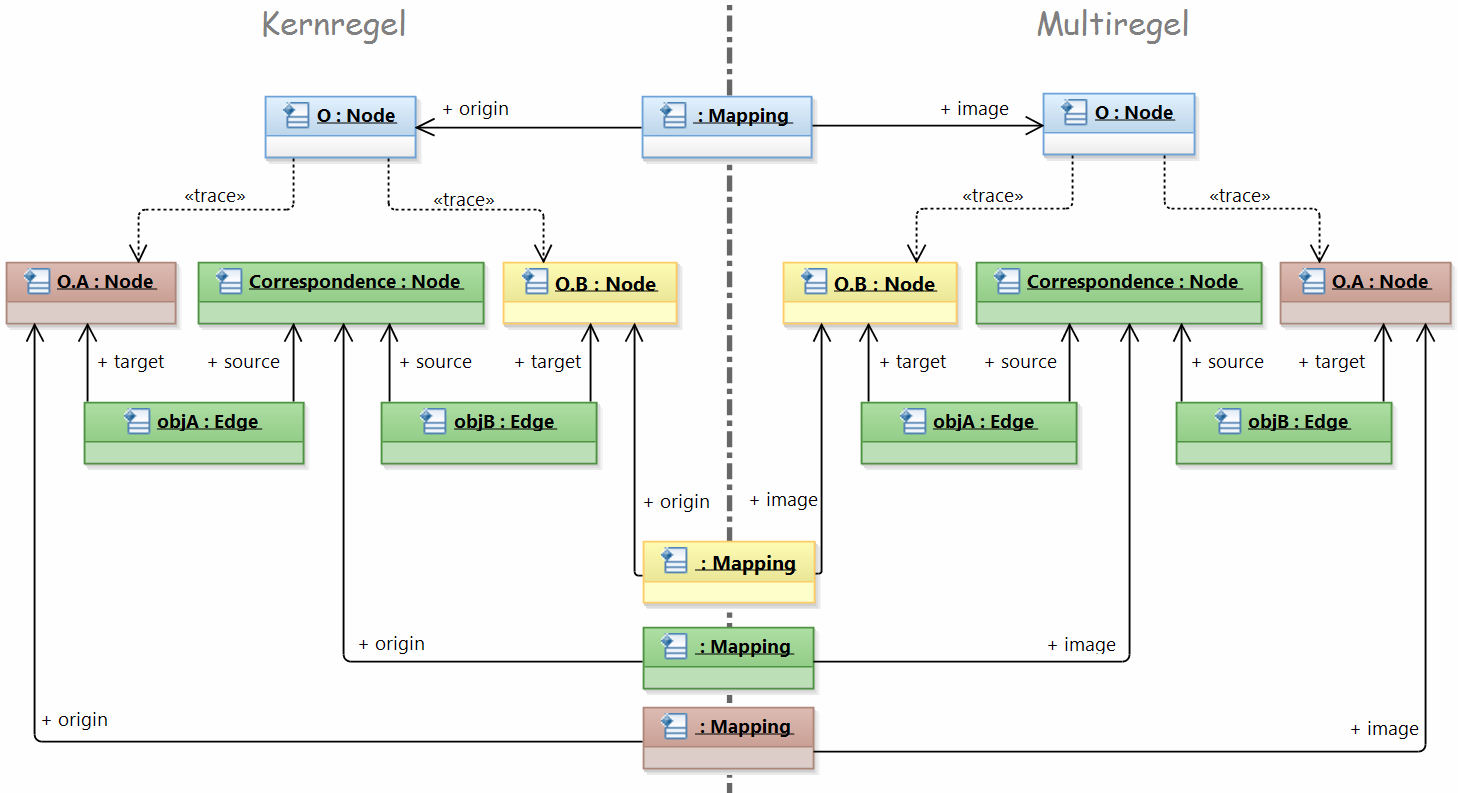
\includegraphics[width=1.0\textwidth]{images/amalgamation_mapping.png}
  \caption{Amalgamation Mapping (LHS bzw. RHS Correspondence-Pattern)}
  \label{fig:amalgamation_mapping}
\end{figure}

Um die Mappings der Erkennungsregel zu erzeugen, werden die Mappings der Editierregel zunächst einem
bestimmten Generierungsmuster zugeordnet. Mappings von \texttt{<<preserve>>} Knoten werden dem
Correspondence-Pattern, Mappings von \texttt{<<delete>>} Knoten werden dem Remove-Object-Pattern und
Mappings von \texttt{<<create>>} Knoten werden dem Add-Object-Pattern zugeordnet. Zu jedem Mapping
der Editierregel können nun über die Traces (Abschnitt \ref{traces}) die entsprechenden Modell A und
B Knoten der Erkennungsregel zugeordnet und das entsprechende Mapping angelegt werden. Anschließend
werden noch die zu den jeweiligen Mustern gehörenden Änderungsknoten bzw.
Correspondence-Knoten gemappt.

Abbildung \ref{fig:amalgamation_mapping} demonstriert diesen Vorgang für zwei \texttt{<<preserve>>}
Knoten \textit{O} einer Amalgamation Editierregel. In der Abbildung wird nur eine der beiden Seiten
der Regel dargestellt. Für alle \texttt{<<preserve>>} Knoten unterscheidet sich aber die LHS nicht
von der RHS. Wie zu sehen ist, sind die Knoten \textit{O} über ein Mapping verbunden. Von beiden
Knoten sind dann über die Traces die entsprechenden Erkennungsregel Knoten zu erreichen, die
aufeinander gemappt werden müssen. Die beiden Correspondence-Knoten sind über die Kanten
\texttt{objA} und \texttt{objB} zu erreichen und müssen ebenfalls gemappt werden.

Die Typknoten des Add/Remove-Object und Attribute-Value-Change-Patterns lassen sich relativ leicht
zuordnen, da diese per Defintion in der Erkennungsregel eindeutig sein müssen. Somit können immer
die gleichen Typknoten aus Kern- und Multiregel aufeinander gemappt werden.

Der Änderungsknoten eines Add-Reference, Remove-Reference oder Attribute-Value-Change-Patterns kann
immer dann zwischen Kern- und Multiregel gemappt werden, wenn die Typknoten (\texttt{type}) und
Modell Knoten (\texttt{src, tgt}) des Musters ebenfallls aufeinander gemappt wurden.

Damit später nur ein Semantic-Change-Set für die Amalgamation Unit erzeugt wird, müssen auch
die Semantic-Change-Set- und Differenzknoten gemappt werden.

\section{Generierung als Higher-Order-Transformation}

Neben der in Java implementierten Version der Erkennungsregel Generierung wurde der Algorithmus
auch als Henshin Transformation angelegt. Da Henshin selbst auf Ecore basiert, ist es technisch
problemlos möglich ein Henshin Transformationssystem wieder durch ein anderes
Henshin Transformationssystem zu transformieren. Man spricht in diesem Fall auch von einer
Higher-Order-Transformation (HOT) \cite{TJF09}. Dies wird in Abbildung \ref{fig:hot} illustriert.
Hier ist zu sehen, dass sowohl Eingabe (Editierregel) als auch Ausgabe (Erkennungsregel) der HOT
\textit{editR2recognitionR} ein Henshin Transformationssystem ist.

\begin{figure}[htb]
  \centering
  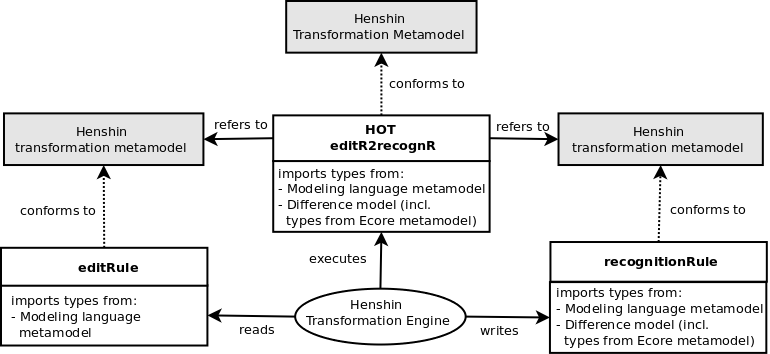
\includegraphics[width=1.0\textwidth]{images/hot_overview.png}
  \caption{Higher-Order-Transformation: Editierregel $\to$ Erkennungsregel}
  \label{fig:hot}
\end{figure}

Um die einzelnen Regeln möglichst noch überschaubar und grafisch darstellbar zu halten, wurde der
Algorithmus in fünf Phasen unterteilt. Dies hat außerdem den Vorteil, dass die Regeln
nachvollziehbar und besser wartbar bleiben. Die sequentielle Abarbeitung dieser Phasen ist in
Abbildung \ref{fig:hot_main_unit} in Form von Henshin Units zu
sehen\footnote{\parbox[t]{\linewidth}{Das vollständige Transformationssystem ist verfügbar unter:
http://pi.informatik.uni-siegen.de/ Projekte/sidiff/pipeline/semantic-lifting/hot/index.htm}}.

\begin{figure}[h!]
  \centering
  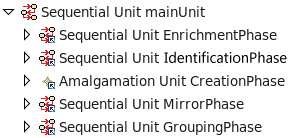
\includegraphics[scale=0.8]{images/hot_main_unit.png}
  \caption{Henshin Main-Unit}
  \label{fig:hot_main_unit}
\end{figure}

Das Problem besteht darin, dass in den meisten Fällen für die Generierung der Muster immer die
rechte und linke Seite der Editierregel betrachtet werden muss und aus diesen Informationen dann
wieder ein rechter und linker Teil der Erkennungsregel resultiert. Auf Grund der Beschaffenheit des
Henshin Metamodells \ref{fig:henshin_metamodel} müssten bei einer direkten Generierung der
beschriebenen Muster häufig sehr viele Objekte gleichzeitig betrachtet werden.

Grundsätzlich ist es in Henshin schwierig, Informationen innerhalb des Transformationssystems
temporär zwischen zu speichern. Um die Information zwischen den verschiedenen Regeln weiter zu
reichen, wird ein für diesen Zweck angelegtes Ecore Modell als Hilfsstruktur verwendet, das s.g.
\textbf{Lifting-Modell}. Wie in Abbildung \ref{fig:lifting_model} zu sehen ist, gibt es eine
zentrale Klasse \texttt{Edit2Recognition}, die alle benötigten Information während der
Transformation verwaltet. Als Startkonfiguration für die Transformation \textit{editR2recognitionR}
wird ein Objekt der Klasse \texttt{Edit2Recognition} mit der Editierregel und einer leeren
Erkennungsregel initialisiert.

\begin{figure}[h!]
  \centering
  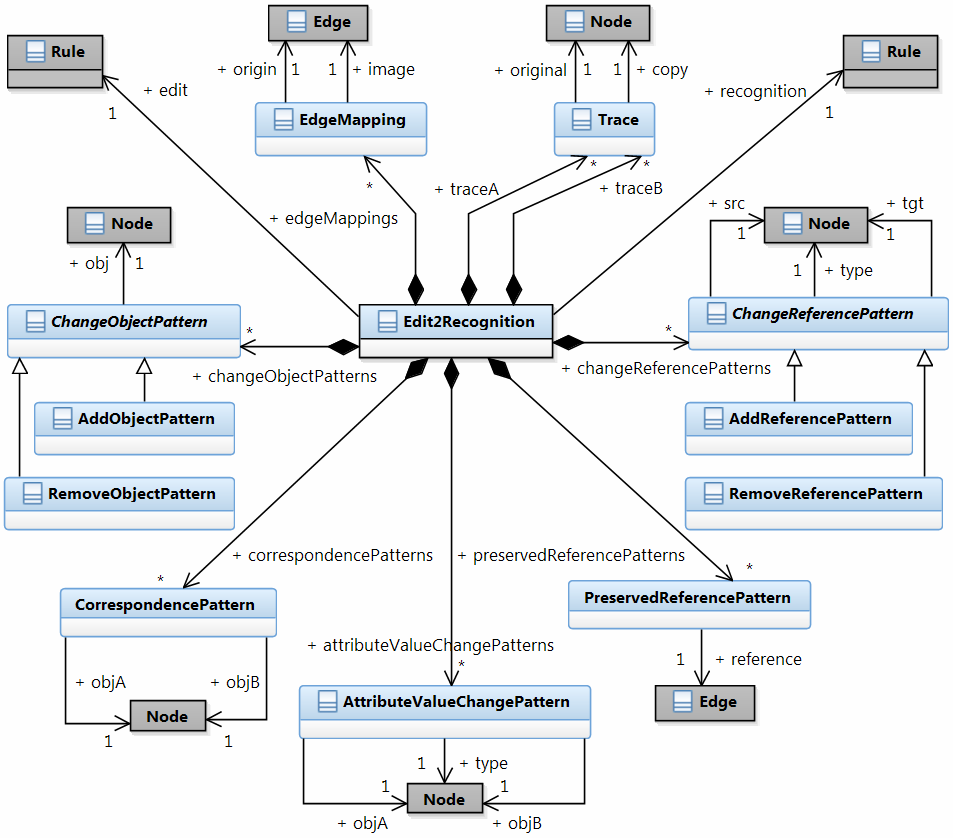
\includegraphics[width=1.0\textwidth]{images/lifting_model.png}
  \caption{Lifting-Modell}
  \label{fig:lifting_model}
\end{figure}

\subsection{Enrichment-Phase}

Die erste Regel (\texttt{Create-Implicite-Edge}) des Transformationssystems wird direkt auf die
Editierregel angewandt. Hierdurch werden die zuvor beschriebenen impliziten Kanten (Abschnitt
\ref{implicit_edge}) in die Editierregel eingefügt.

Der nächst Schritt dient dazu, den Umgang mit dem Transformationssystem  der Editierregel  zu
erleichtern. Für \texttt{<<preserve>>}  Knoten werden explizit Mappings für die Graphen angelegt,
für Kanten ist dies nicht der Fall. Um später einfacher herausfinden zu können, ob eine Kante
\texttt{<<preserve>>} ist, wird durch die Regel \texttt{Map-Preserved-Edge} für jede Kante, die
sowohl auf der rechten als auch auf der linken Seite einer Regel vorkommt, ein Edge-Mapping
angelegt. Das Edge-Mapping wird durch das Lifting-Modell abgespeichert und ist somit für alle
weiteren Regeln verfügbar.

\begin{figure}[h!]
  \centering
  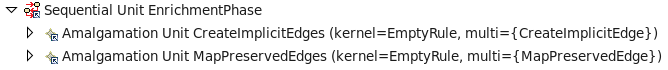
\includegraphics[scale=0.8]{images/hot_enrichment_unit.png}
  \caption{Henshin Enrichment-Unit}
  \label{fig:hot_enrichment_unit}
\end{figure}

Wie in Abbildung \ref{fig:hot_enrichment_unit} zu sehen ist, müssen erst alle impliziten Kanten
angelegt werden bevor das Mapping der Kanten gestartet werden kann. Durch die Verwendung von
Amalgamation Units werden die beiden Regeln  jeweils parallel auf alle Matches angewandt. Die
leere Kernregel bewirkt, dass die Mulitregeln für jeden gefundenen Match einmal in die temporär
angelegte Amalgamation Regel kopiert werden.

\subsection{Identification-Phase} 

In der ersten Phase werden die Informationen für die einzelnen Generierungsmuster gesammelt. Ziel
ist es zunächst einmal nur die wirklich benötigten Informationen abzuspeichern, um die einzelnen
Regeln möglichst klein zu halten. Im Lifting-Modell gibt es daher eine Klasse für jedes
Generierungsmuster (Abschnitt \ref{patterns}). Genauso existiert eine Matching-Regel für jedes
Muster. Für jeden Match, der in der Editierregel gefunden wird, wird dann ein Objekt der
entsprechenden Klasse im Lifting-Modell angelegt.

Da sich die Modell A und B Knoten in den verschiedenen Mustern überschneiden, muss es eine
Möglichkeit geben einen Erkennungsregel Knoten einem entsprechenden Knoten der Editierregel
zuzuordnen. Diese Aufgabe wird durch die bereits erwähnten Traces (Abschnitt \ref{traces}) erledigt. Ein
Trace ordnet immer einem Knoten der Editierregel (\texttt{original}) einen Knoten der Erkennungsregel (\texttt{copy})
zu. Die Traces werden nach Modell A und B Knoten unterschieden im Lifting-Modell abgespeichert.

Das anlegen aller Modell A und B Knoten und Traces erfolgt in der ersten Unterphase der
Identification-Phase (Abbildung \ref{fig:hot_identification_and_create_unit}
IdentificationPhase01 (links)). Die Überschneidenden Muster werden erste in der zweiter
Unterphase (Abbildung \ref{fig:hot_identification_and_create_unit} IdentificationPhase02 (links)) angelegt.

\begin{figure}[h!]
  \centering
  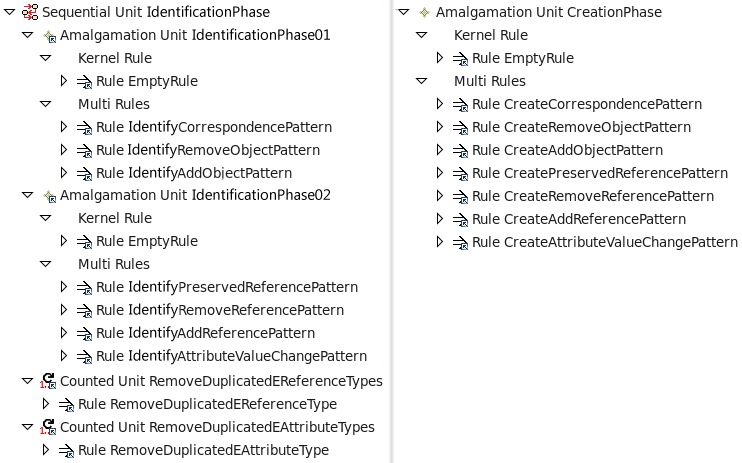
\includegraphics[width=1.0\textwidth]{images/hot_identification_and_create_unit.png}
  \caption{Henshin Identification- und Create-Unit}
  \label{fig:hot_identification_and_create_unit}
\end{figure}

Die Typknoten \texttt{ChangeReferencePattern.type, AttributeValueChangePattern. type} werden beim
ausführen der Amalgamation Unit der Muster Remove/Add-Reference und Attribute-Value-Change-Pattern
parallel angelegt. Wie in Abschnitt \ref{typknoten} beschrieben, müssen diese Knoten aber in der
Erkennungsregel eindeutig sein. Bis zu diesem Zeitpunkt ist es noch möglich, dass ein Typknoten
mehrfach in den im Lifting-Modell angelegten Muster Objekten vorkommt. Um dieses Problem zu beheben,
werden durch die Regeln \texttt{Remove-Duplicated-Types} nachträglich alle duplizierten Typknoten
aus den Muster Objekten entfernt und alle \texttt{type} Kanten auf eine einzelne Instanz gesetzt.
Dazu werden die beiden Regeln, wie in Abbildung \ref{fig:hot_identification_and_create_unit} zu
sehen, als Counted-Unit (\texttt{count = -1}) solange ausgeführt bis kein Duplikat mehr gefunden
wird.

Betrachtet man eine Erkennungsregel, so sind der linke und rechte Graph der Regel, abgesehen vom
Semantic-Change-Set, identisch (\texttt{<<preserve>>}). Es reicht daher aus zunächst nur einen
einfachen Graphen zu erzeugen. Dieser Graph kann dann später einer Seite der Regel zugeordnet und
auf die andere Seite gespiegelt bzw. kopiert werden.

\subsection{Create-Phase} 

In der nächsten Phase werden für alle gesammelten Muster im Lifting-Modell die noch fehlenden
Änderungsknoten (\texttt{Correspondence, Add/Remove-Object, Add/Remove-Re"-ference}) und die dazu
gehörigen Kanten eingefügt. Außerdem werden sämtliche Knoten und Kanten einem Graphen und der Graph
der linken Seite der Regel zugeordnet. Wie in Abbildung \ref{fig:hot_identification_and_create_unit}
(rechts) zu sehen, ist dieser Prozess für alle Muster voneinander unabhängig und kann damit
parallel ausgeführt werden.

\subsection{Mirror-Phase} 

Da bisher nur der linke Teil der Erkennungsregel angelegt wurde, muss im nächsten Schritt der linke
Graph vollständig in den rechten Graph kopiert werden. Zusätzlich müssen zwischen allen Knoten der
linken und rechten Seite Mappings angelegt werden. Hierzu gibt es je eine Regel für Knoten, Kanten
und Attribute. Die Abarbeitung der Regeln ist in Abbildung \ref{fig:hot_mirror and_grouping_unit}
(links) zu sehen.

% \begin{figure}[h!]
%   \centering
%   \includegraphics[scale=0.8]{images/hot_mirror_unit.png}
%   \caption{Henshin Mirror-Unit}
%   \label{fig:hot_mirror_unit}
% \end{figure}

\subsection{Grouping-Phase} 

Nachdem der \texttt{<<preserve>>} Teil der Erkennungsregel erzeugt wurde, muss abschließend noch das
Semantic-Change-Set erzeugt und anschließend mit allen low-level Änderungsknoten verbunden werden.
Siehe Abbildung \ref{fig:hot_mirror and_grouping_unit} (rechts).

\begin{figure}[h!]
  \centering
  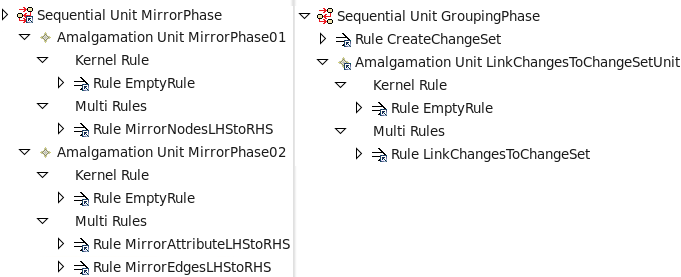
\includegraphics[scale=0.8]{images/hot_mirror_and_grouping_unit.png}
  \caption{Henshin Mirror- und Grouping-Unit}
  \label{fig:hot_mirror and_grouping_unit}
\end{figure}

\section{Vergleich von HOT und Java Implementierung}

% A very brief specification sketch of designing \textit{editR2recognR} as direct manipulation
% approach in imperative logic \cite{CzH2006IBM} is given in \cite{KeKT2011ASE}. We implemented the
% direct manipulation in Java\footnote{The source code is freely available at:
% http://pi.informatik.uni-siegen.de/Projekte/sidiff/pipeline/semantic-lifting/hot/index.htm}
% independently from our implementation in Henshin. A comparison of both implementation design
% reveals, that almost the same ``functions'' are used (s.
% Table \ref{tab:java-comparison}).
% 
% A design pattern that can be observed for the Henshin-based realization is the sequential enrichment
% of helper data. This is used to ``emulate'' procedure calls providing return values of complex data
% types. For example, the creation of atomic change patterns can be decomposed into two logical
% functions: Firstly, their cause have to be detected by an analysis of the edit rule before the
% pattern specification is actually synthesized within the recognition rule. For a concrete type of
% atomic change pattern, e.g. the correspondence pattern, this is implemented straight-forward in
% Java: The method \texttt{createCorrespondencePatterns()} simply calls the utility method
% \texttt{getLHSIntersectRHSNodes()}, which implements a query that returns the ``preserved'' nodes of
% an edit rule. In Henshin, the same utility function is realized by the rule
% \texttt{IdentifyCorrespondencePattern} which creates helper data being later used by the rule
% \texttt{CreateCorrespondencePattern}.

Die Implementierung des Erkennungsregel Generators unter Java\footnote{Die Quellcodes sind frei
verfügbar unter: http://pi.informatik.uni-siegen.de/Projekte/sidiff/pipeline/
semantic-lifting/hot/index.htm} wurde unabhängig von der Henshin Implementierung geschrieben. Ein
Vergleich beider Ansätze zeigt aber einige Parallelen auf. Wie in Tabelle \ref{tab:java-comparison}
zu sehen ist, ist die Aufteilungen der einzelnen Funktionalitäten sehr ähnlich. Ein technischer
Unterschied zwischen einem prozeduralen Aufruf in Java und dem Ausführen einer Regel in Henshin
besteht darin, dass eine Henshin Regel keine komplexen Datentypen durch einen Rückgabewert an
andere Regeln weiterreichen kann.

Ein Entwurfsmuster, das sich in der Henshin-basierten Realisierung beobachten lässt, ist die
sequentielle Anreicherung des Lifting-Modells, das als Hilfsstruktur verwendet wird. Die
Hilfsstruktur wird verwendet, um ähnlich wie bei prozeduralen Aufrufen in Java komplexe Datentypen
durch eine Regel zurückzugeben. Dies lässt sich am Beispiel der einzelnen Generierungsmuster
beobachten. Ein Muster wird hier in zwei aufeinander folgenden Schritten erzeugt. Zunächst wird die
Editierregel auf das Vorkommen eines bestimmten Musters geprüft und erst im nächsten Schritt werden
die daraus resultierenden Muster in der Erkennungsregel angelegt. Dieses Vorgehen findet sich
genauso in der Java Implementierung wieder. Alle Correspondece-Patterns werden in Java mit dem
Aufruf der Funktion \texttt{createCorrespondencePatterns()} erzeugt. Um alle Teile einer
Editierregel zu identifizieren, auf die das Muster angewendet werden soll, wird dann zunächst die
Funktion \texttt{getLHSIntersectRHSNodes()} aufgerufen, welche alle \texttt{<<preserve>>} Knoten der
Editierregel zurückliefert. In Henshin wird die gleiche Funktionalität durch die Regeln
\texttt{Identify-Correspondence-Pattern} zum Identifizieren aller \texttt{<<preserve>>} Knoten und
\texttt{Create-Correspondence-Pattern} zum Anlegen aller Muster ausgeführt.

\begin{table}[h!]
\centering
\caption{Vergleich von HOT und Java Implementierung}
\begin{tabular}{llcl}
\toprule
\textbf{Phase} \ & \textbf{Henshin Regel}  & & \textbf{Java Methode / Utility} \\
\cmidrule{1-4}
EP: & CreateImplicitEdge & & createImplicitEdges() \\
& MapPreservedEdge & & isEdgeMapped() \\

IP: & MatchCorrespondencePattern & & getLHSIntersectRHSNodes() \\
& IdentifyAddObjectPattern & & getRHSMinusLHSNodes() \\
& \multicolumn{1}{c}{\vdots} & & \multicolumn{1}{c}{\vdots} \\
& RemoveDuplicatedEReferenceTypes & & -  \\
& RemoveDuplicatedEAttributeTypes & & -  \\

CP: & CreateCorrespondencePattern & & createCorrespondencePatterns()  \\
& CreateAddObjectPattern & & createAddObjectPatterns()  \\
& \multicolumn{1}{c}{\vdots} & & \multicolumn{1}{c}{\vdots} \\

MP: & MirrorNodesLHStoRHS & & - \\
& MirrorAttributeLHStoRHS & & - \\
& MirrorEdgesLHStoRHS & & - \\

GP: & CreateChangeSet & & \multirow{2}{*}{createChangeSet()} \\
& LinkChangesToChangeSet & & \\
\cmidrule{2-4}
& - & & ModelHelper.java \\
& - & & ModelHelperEx.java \\
& - & & NodePair.java \\
\bottomrule
\end{tabular}
  \label{tab:java-comparison}
\end{table}

Die beiden Regeln \texttt{Remove-Duplicated-EReference-Types} und
\texttt{Remove-Duplicated"-EAttribute-Types} haben keine entsprechenden Java Methoden. Der
Unterschied in den Implementierungen besteht darin, dass die Muster, in denen die Typknoten erkannt
bzw. erzeugt werden in Henshin parallel und in Java sequentiell abgearbeitet werden. Daher kann in
Java die Existenz eines Typknoten direkt beim Anlegen des Musters überprüft werden (Zeile 258, 340
und 405 in \texttt{EditRule2RecognitionRule.java}). In Henshin kann dies durch die Parallelität erst
nachträglich erledigt werden. Grundsätzlich wäre es aber auch möglich, den gleichen Ablauf in
Henshin über ein \texttt{If then else} Konstrukt zu realisieren.

Während in Henshin alle  \texttt{<<preserve>>} Anteile über die Regeln
\texttt{Mirror-Nodes-LHS-to"-RHS}, \texttt{Mirror-Attribute-LHS-to-RHS} und
\texttt{Mirror-Edges-LHS-to-RHS} abgearbeitet werden, wird die gleiche Funktionalität in Java über
Hilfsfunktionen und Hilfsstrukturen geregelt. Die Utility Funktion \texttt{createPreservedNode()}
der Klasse \texttt{HenshinRuleAnalysis"-UtilEx} und die Hilfsstruktur \texttt{NodePair} werden dem
Programmierer zur Verfügung gestellt um die LHS und RHS Verwaltung von \texttt{<<preserve>>} Knoten
transparent zu handhaben.
 
% Two Henshin rules that do not have any corresponding Java method implementing the same functionality
% are \texttt{RemoveDuplicatedEReferenceTypes} and \texttt{RemoveDuplicatedEAttributeTypes} In terms
% of the Java implementation, duplicate type nodes are never created because a simple condition checks
% whether these type nodes already exist when an atomic change pattern is synthesized (cf. lines 258,
% 340 and 405 in \texttt{EditRule2RecognitionRule.java}). In Henshin, the same behavior could be
% realized using conditional units and implementing a loop processing instead of a parallel creation
% of atomic change patterns. In this case, \texttt{RemoveDuplicatedEReferenceTypes} and
% \texttt{RemoveDuplicatedEAttributeTypes} would be obsolete. However, the total number of rules
% needed by this transformation design would be significantly higher: For each rule of the
% identification phase, three rules would be required, i.e. ``if rule'', ``then rule'' and ``else
% rule'' of the respective conditional unit.
% 
% Further Henshin rules which have no corresponding Java methods implementing the same function are
% \texttt{MirrorNodesLHStoRHS}, \texttt{MirrorAttributeLHStoRHS} and \texttt{MirrorEdgesLHStoRHS},
% which facilitate the output rule synthesis; initially only the LHS of the output recognition rule
% has to be synthesized which is later mirrored onto the RHS. In Java, the consistent handling of LHS
% and RHS graphs of a recognition rule is implemented using data abstractions.
% These data abstractions provide a high-level API to manipulate internal, fine-grained
% representations of Henshin rules. For example, the utility function \texttt{createPreservedNode()}
% of class \texttt{HenshinRuleAnalysisUtilEx} and the wrapper class \texttt{NodePair} are provided in
% order to encapsulate preserved nodes: Creation and management of LHS node, RHS node and the
% according mapping are handled transparently to a programmer.

Dieser Vergleich zeigt, dass Entwurfsmuster und Techniken der prozeduralen Programmierung auch im
Bereich der Modelltransformation hilfreich eingesetzt werden können. Übertragen lassen sich diese
durch die Aufteilung der verschiedenen Funktionalität auf einzelne Regeln und durch die Verwendung
von Hilfsstrukturen, um komplexe Datentypen zu handhaben. Die Technik von LHS zu RHS zu spiegeln, um
\texttt{<<preserve>>} Knoten anzulegen, ist relativ speziell, lässt sich aber auch auf ähnliche
Mustererkennungsprobleme übertragen.

% Instead, our rule-based transformation design based on EMF Henshin reveals that patterns that are
% known form procedural programming can help to structure the transformation design.
% Utility functions providing structurally complex return types can be realized by the definition of
% an intermediate helper structure. This pattern can be generalized and applied to all types of
% rule-based transformations. Two other patterns that are used specifically apply to higher-order
% transformations: Firstly, providing the explicit information of preserved edges facilitates queries
% on the rule serving as input of the HOT. Secondly, the mirroring of preserved parts from LHS to RHS
% facilitates the output rule synthesis. The second pattern is very specific to the transformation
% domain described in this paper as most parts of a recognition rule are preserved. However, it can be
% generalized to all HOTs generating transformation rules that are mainly used for pattern matching
% purposes.